\documentclass[12pt]{beamer}
\usetheme{CambridgeUS}
\usecolortheme{lily}
\usepackage{extsizes}
\usepackage{amsmath}
\usepackage{setspace}
\usepackage{commath}
\usepackage{graphicx}
\geometry{margin=0.0in}
\title{debuginfod}
\subtitle{and its interaction with the 
Yocto Project}
\author{Dylan Garza}
\date{\today}

\begin{document}

\frame{\titlepage}

\begin{frame}
   \frametitle{ debuginfod}
   \begin{itemize}
      \item What is debuginfod?
      debuginfod is a daemon turns a machine that
      holds debug artifacts into file server for
      easier debugging. \\
      \vspace{.5cm}
      \item Why use it?
      Debug info is too big to be stored locally
      on the target devices. Different versions 
      of binaries exist, storing and searching 
      for debug artifacts manually is too slow.
   \end{itemize}
\end{frame}

\begin{frame}[fragile]
   \frametitle{ Installing debuginfod}
   \vspace{-1cm}
   \noindent
   There are two ways to install on a Ubuntu machine:
   \begin{itemize}
      \item Upgrade to Ubuntu 22.04
      \item append the impish package to \verb|/etc/apt/sources.list|
   \end{itemize}
   %add image here of line appended
\end{frame}

\begin{frame}[fragile]
   \frametitle{Setting up and using debuginfod}
   \vspace{-1cm}
   Starting the debuginfod server:
   \begin{itemize}
      \item To start the file server, simply run \verb|debuginfod -F|. 
         Different arguments will search for different debug artifacts (\verb|-F -R -U|)
      \item Providing a path to a directory will point debuginfod where to scan for the debug artifacts.
      \item To set a rescan time, provide \verb|-t [time in seconds]|
   \end{itemize}
\end{frame}

\begin{frame}[fragile]
   \frametitle{ Setting up and using debuginfod (cont.)}
   \vspace{-1cm}
   On the host machine:
   \begin{itemize}
      \item set environment variable \verb|DEBUGINFOD_URLS| to the ip address 
         of the file server, prefixed by \verb|http://| and suffixed by the 
         port number defaulted to \verb|:8002|, which can be changed by \verb|-p [port num]|
   \end{itemize}
   \begin{verbatim}
    export DEBUGINFOD_URLS="http://ip_addr:8002"
    \end{verbatim}


\end{frame}

\begin{frame}[fragile]
   \frametitle{ Federating debuginfod servers}
   debuginfod servers can act as a host machine and query other servers
   %include image
   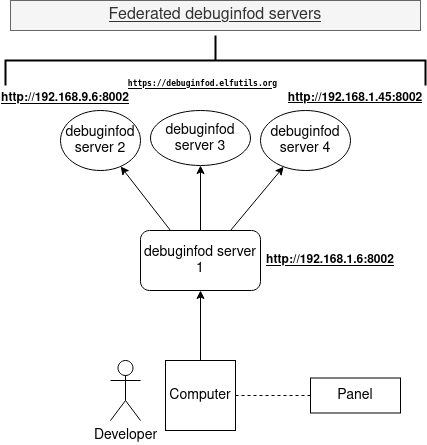
\includegraphics[scale=0.45]{federeated_servers.png}
   %include diagram
\end{frame}

\begin{frame}
   \frametitle{ Federeating debuginfod servers (cont.) }
   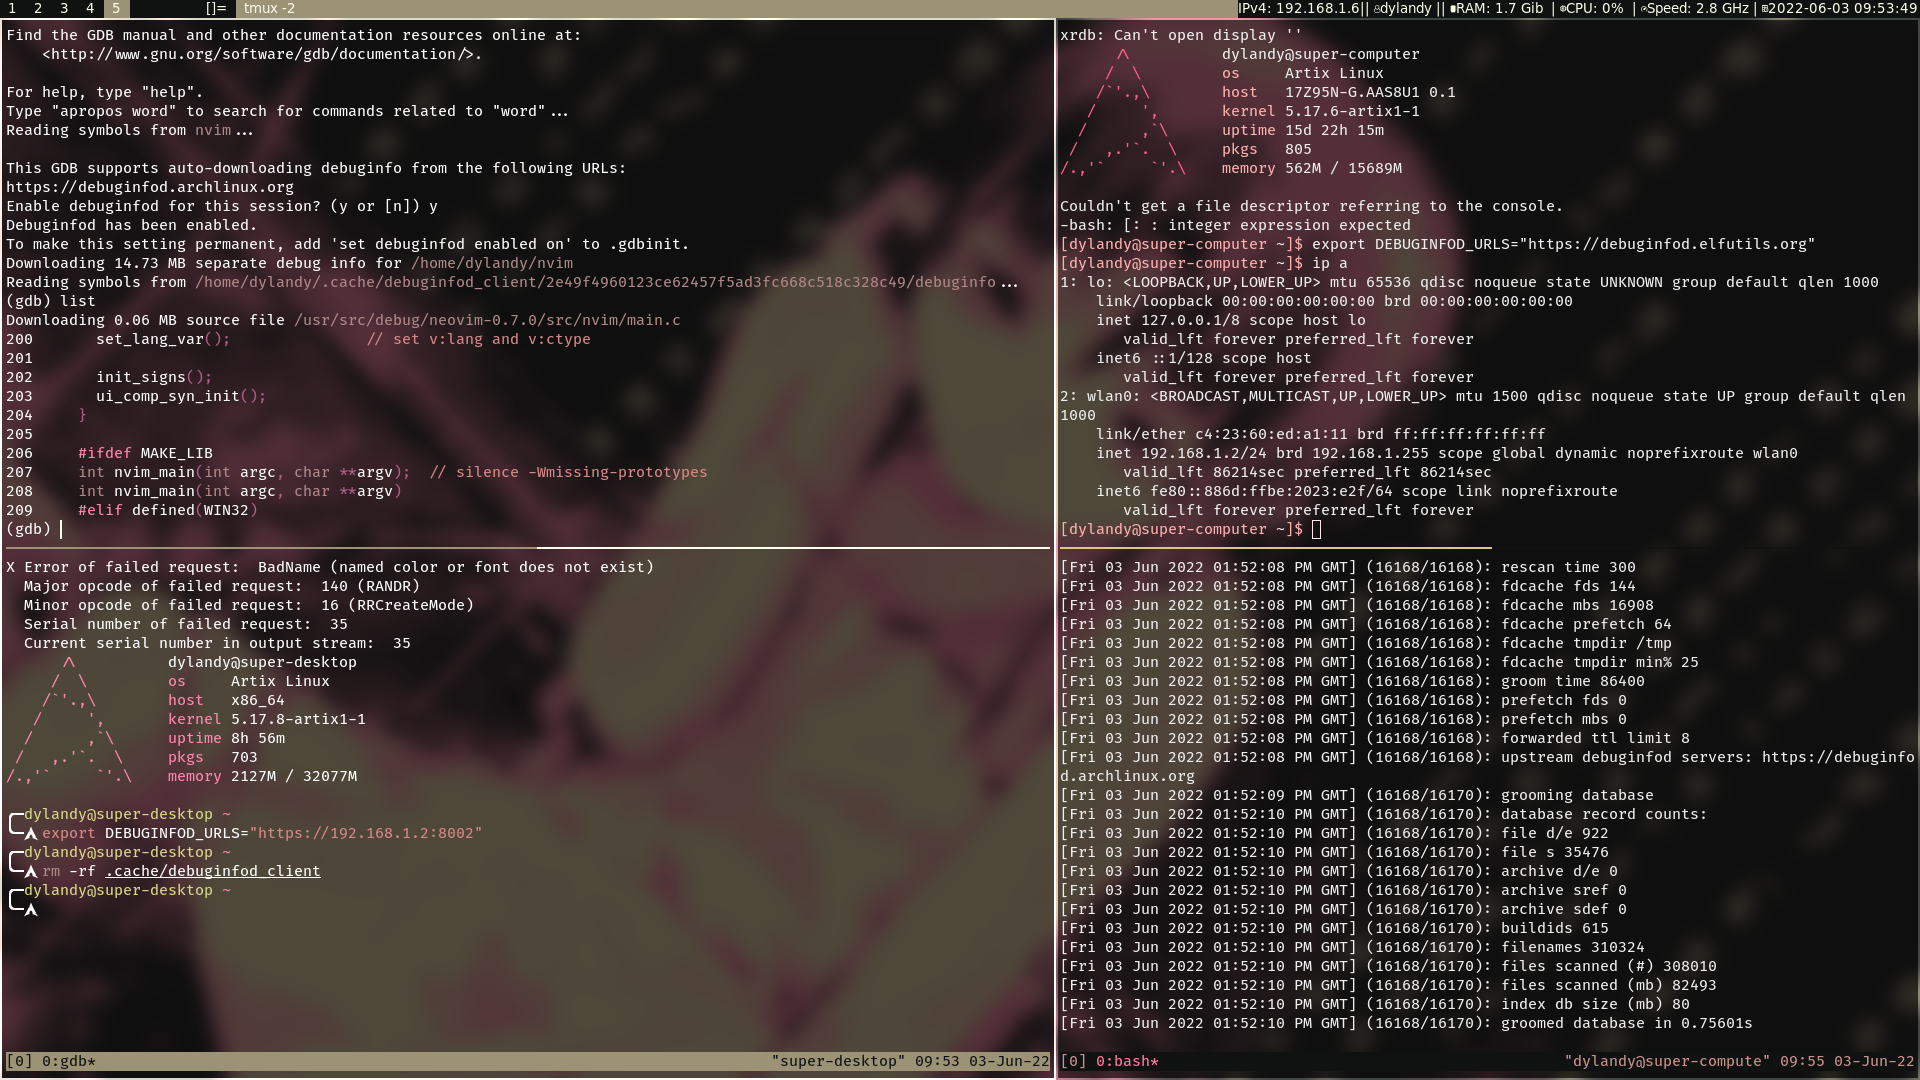
\includegraphics[scale=.1775]{federated_ss.png}
\end{frame}

\begin{frame}
   \frametitle{ Demo}
\end{frame}

\begin{frame}[fragile]
   \frametitle{ debuginfod with the Yocto Project}
   For versions after 3.4(honister) only 2 changes are needed for debuginfod
   to work on a build. Append the following the \verb|local.conf|:
   \begin{small}
   \begin{enumerate}
      \item \verb|PACKAGE_CONFIG_pn-elfutils-native="debuginfod libdebuginfod"|
      \item \verb|DISTROFEATURES += "debuginfod"|
   \end{enumerate}
   \end{small}
   Yocto Project has built in script for debuginfod to eliminate compatability issues. 
\end{frame}

\begin{frame}[fragile]
   \frametitle{ debuginfod-find}
   Command apart of elfutils, it performs debuginfod server querying without gdb. Can query for
   debuginfo, executables, and sources. 
   \begin{tiny}
   \begin{verbatim}
   debuginfod-find [debuginfo/executable/source] [path/to/file or Build-ID] [path/to/source]
   \end{verbatim}
   \end{tiny}
   If the path to the source is not known, but debug info is available, use the \verb|list| command
   under gdb to provide source path. 

\end{frame}

\begin{frame}
   \frametitle{ Demo }
\end{frame}


\end{document}
